%%==================================================
%% chapter01.tex for BIT Master Thesis
%% modified by pinren lu
%% version: 0.1
%% last update: Dec 25th, 2016
%%==================================================

\chapter{模型改写文本检测方法}
\label{chap:method}

\section{引言}
\label{sec:method-intro}

在第三章中,本文详细介绍了模型改写文本检测数据集(TOSWT 数据集)的构造方法,强调了数据清洗、句子分割以及利用大型语言模型进行文本改写的重要性。这一过程为后续的文本检测任务奠定了坚实的基础。在本章中,我们将深入探讨模型改写文本检测的方法,着重分析基于预训练模型的技术路线,并阐明实验设计及其结果。

随着人工智能技术的飞速发展,尤其是大型语言模型的广泛应用,文本生成的质量和复杂性显著提升。这使得传统的文本检测方法面临新的挑战,尤其是在识别和追踪人工智能生成文本方面。因此,开发有效的模型改写文本检测方法,成为了当前自然语言处理领域的重要研究方向。通过构建有效的检测模型,我们能够更好地识别出文本中可能的人工智能生成部分,从而为教育领域提供支持。

本章的核心目标是基于句子级文本检测来完成文档级的文本检测。方法首先将
输入文档划分为独立的句子单元,识别局部改写特征,并计算计算句子贡献度,并将各句子的检测置信度与其对应的注意力权重进行矩阵乘法运算,将该贡献度与句子检测结果相乘生成文档级检测得分。

此外,我们将设计一系列实验,以评估所提出的方法在模型改写文本检测中的有效性。这些实验将包括数据集设置、参数配置、评价指标的选择以及对比实验的结果分析。通过这些实验,我们不仅能够验证所提出方法的性能,还能为后续研究提供宝贵的经验和数据支持。

通过本章的研究,我们希望能够为模型改写文本检测领域提供新的思路和方法,推动相关技术的发展与应用。同时,我们也期待这些研究成果能够为教育工作者提供切实可行的解决方案,并启发内容审核人员以及其他相关领域的从业者的应用思路,以应对日益复杂的文本来源问题。

% \section{基于预训练的模型改写文本检测}
% \label{sec:method-pretrain}

% 随着自然语言处理(NLP)技术的不断进步,基于预训练模型的方法在文本分析和理解任务中取得了显著的成功。预训练模型通过在大量文本数据上进行训练,学习到丰富的语言特征和语义信息,这使得它们在特定任务中表现出色。在模型改写文本检测领域,利用这些预训练模型能够有效地识别和追踪文本的来源,尤其是在面对人工智能生成的文本时。

% 预训练模型的核心优势在于其强大的上下文理解能力。与传统的特征工程方法相比,预训练模型能够自动提取文本中的深层次特征,从而提高文本分类和检测的准确性。这一过程通常分为两个阶段:首先是在大规模文本数据上进行无监督预训练,然后在特定任务上进行微调。通过这种方式,模型能够适应不同的文本风格和结构,从而增强其在特定应用场景下的性能。

% 在模型改写文本检测任务中,预训练模型的使用能够帮助我们识别文本中的细微差异,例如句子结构的变化、用词的替换以及语义的调整。这对于判断文本是否经过人工智能模型的改写尤为重要。通过分析文本的上下文信息,预训练模型能够捕捉到潜在的模式和特征,这些模式可能是人类作者与人工智能生成文本之间的显著区别。

% 在上文中,本文介绍了两种流行且被本课题应用的预训练模型:RoBERTa \cite{liu_roberta_2019} 和 DeBERTa \cite{he_deberta_2021, he2023debertav3improvingdebertausing}。这两种模型在文本理解和生成任务中都表现出色,尤其是在文本分类和检测方面,已被广泛应用于多个研究领域。

\section{基于句子级文本检测技术的文档级文本检测方法}
\label{sec:method-sent2arti}

本研究提出了一种层次化文档检测框架,其核心架构如图\ref{fig:method-sent2arti}所示。该方法采用"分而治之"的策略,首先将输入文档通过句子分割模块分解为独立的句子单元。每个句子单元并行送入两个处理通道:第一通道采用冻结参数的DeBERTa-V3-Large模型执行细粒度检测,该模型已在句子级数据上完成微调,能够精准识别局部改写特征;第二通道计算句子贡献度,该贡献度通过多头注意力机制捕获句子间的语义关联强度。最终通过加权融合模块将各句子的检测置信度与其对应的注意力权重进行矩阵乘法运算,采用线性层降维后得到句子贡献度,最后将该贡献度与句子检测结果相乘生成文档级检测得分。这种设计实现了三个关键突破:(1)通过分层处理解决长文本建模难题;(2)引入注意力机制保留上下文语义;(3)建立端到端的可微分计算流程。

\begin{figure*}[htbp]
    \centering
    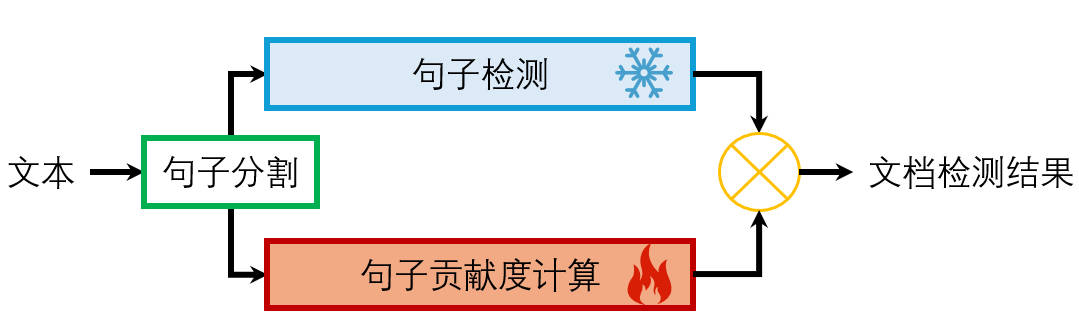
\includegraphics[width=0.9\textwidth]{figures/sent2arti.jpg}
    \caption{基于句子级文本检测技术的文档级文本检测方法}
    \label{fig:method-sent2arti}
\end{figure*}

为验证所提方法的优越性,本文也设计了系统的对比实验方案。基线模型包括三种典型架构:(1)直接迁移模型,将在句子级数据微调的 DeBERTa-V3-Large 模型直接应用于文档检测,用于验证领域适配性问题;(2)朴素加权模型,采用等权重策略(固定注意力值为1)处理所有句子,作为注意力机制有效性的对照基准;(3)长度加权模型,将句子长度作为权重系数,验证表面特征的有效性。所有对比模型均采用相同的训练/测试数据划分。

接下来将介绍基于句子级文本检测技术的文档级文本检测方法的三大模块,分别为句子分割模块、句子贡献度计算模块和句子检测模块。

\subsection{句子分割}

本节句子分割应用 \ref{sec:TOSWT-gen-sentence_splitter} 节中介绍的句子分割工具。这种分割方法能够将输入的文本字符串精准地分割成独立的句子,返回一个结构化的句子列表。其核心原理是通过一系列精心设计的正则表达式和逻辑规则来识别句子边界,有效处理各种复杂的标点符号和特殊情况。

该句子分割器的处理流程分为四个关键步骤。首先进行输入验证,检查输入文本是否为None或空字符串,确保对无效输入的优雅处理。其次,通过多个正则表达式规则在句子边界处插入换行符作为分隔符,这些规则涵盖了非句号结束标记、多重句号、标点符号后接引号或括号等多种复杂情况。然后,系统会进一步处理特殊标点情况,包括识别荣誉称谓、大写字母缩写和数字相关符号等,避免错误分割。最后,系统会清理文本中的多余空格和换行符,确保输出格式整洁。

\subsection{句子贡献度计算}

句子贡献度计算模块的设计旨在通过多头注意力机制捕获句子间的语义关联强度。该模块的核心思想是通过计算句子间的注意力权重,来评估每个句子在整体文本中的重要性和贡献度。句子列表 \( S = [s_1, s_2, \ldots, s_n]^T\) 经过句子贡献度计算模块后得到每一个句子的贡献度 \( \textbf{g} = [g_1, g_2, \ldots, g_n]^T\)。具体过程如图 \ref{fig:method-sent-contribution} 所示。

\begin{figure*}[htbp]
    \centering
    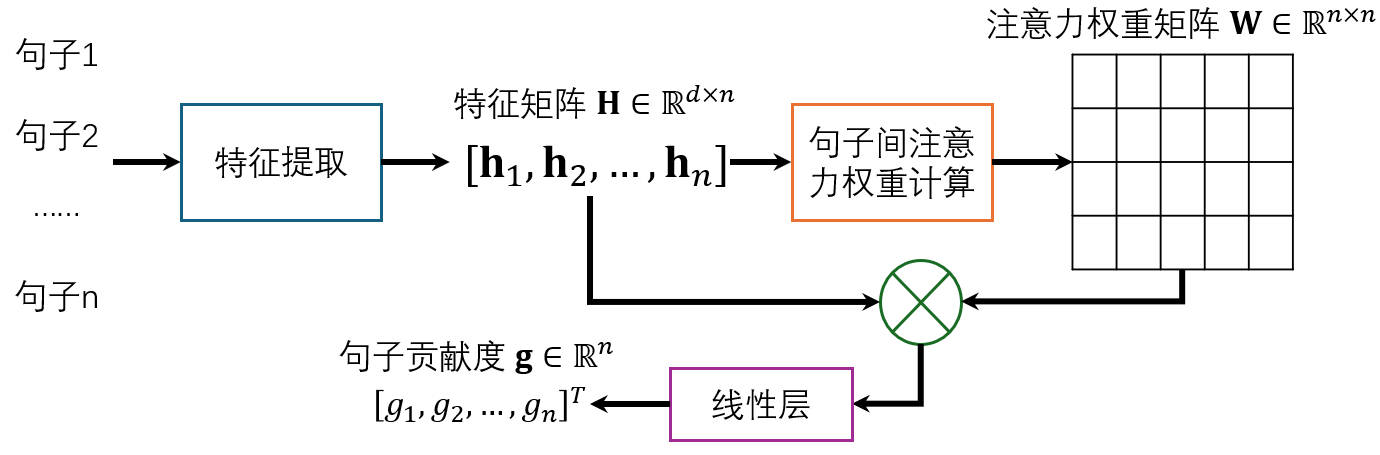
\includegraphics[width=\textwidth]{figures/sent-contribution.jpg}
    \caption{句子贡献度计算}
    \label{fig:method-sent-contribution}
\end{figure*}

具体而言,该模块先将每个句子特征提取:
\begin{equation}
\begin{aligned}
    \textbf{H} = \text{Feature\_Extract}(S)
\end{aligned}
\label{eq:method-sent-contribution-feature}
\end{equation}
其中, \(\textbf{H} \in \mathbb{R}^{d_\text{model} \times n}\) 为句子特征矩阵,\(S = [s_1, s_2, \ldots, s_n]^T\) 为句子列表。接着,计算句子间的注意力权重:
\begin{equation}
\begin{aligned}
    \textbf{W} = \text{Attention}(\textbf{H})
\end{aligned}
\label{eq:method-sent-contribution-attention}
\end{equation}
\(W \in \mathbb{R}^{n \times n}\) 为句子间的注意力权重矩阵。最后,通过特征矩阵 $\textbf{H}$ 与注意力权重矩阵 $\textbf{W}$ 做矩阵相乘运算后使用线性层降维,计算句子贡献度:
\begin{equation}
\begin{aligned}
    \textbf{g} = \text{Linear}(\textbf{HW})
\end{aligned}
\label{eq:method-sent-contribution}
\end{equation}
\(\textbf{g} \in \mathbb{R}^{n}\) 为句子贡献度向量。

在接下来的两节中,本文将详细介绍句子贡献度计算模块中的特征提取(公式 \ref{eq:method-sent-contribution-feature})和句子间注意力权重计算(公式 \ref{eq:method-sent-contribution-attention})的具体实现。

\subsubsection{特征提取}

特征提取模块使用BGE(Bidirectional Generative Encoder)\cite{bge_embedding}作为基座模型。相比BERT,BGE采用RetroMAE非对称自编码架构,通过编码器-解码器的非对称设计强化语义表征能力。其中编码器(BERT-base)接受15-30\%掩码率的输入,专注于捕捉双向上下文;解码器仅使用单层Transformer 解码层,输入掩码率高达50-70\%,用于对遮掩文本进行重建。在训练过程中的编码阶段,模型对输入文本随机进行15\%-30\%的遮掩,然后通过编码得到对应文本的嵌入向量;而在解码阶段,为了提高任务复杂性,文本噪声被进一步加大(掩码比例增加至50\%-70\%),随后通过双流自注意力机制训练解码器从残缺信息中重建完整文本。相比 BERT 仅关注局部词语预测的架构,这种非对称设计能迫使编码器生成更加强大的嵌入向量,对提升模型的语义理解和表征能力效果显著。单个句子的特征提取三个阶段具体实现如图 \ref{fig:method-feature-extract} 所示。

\begin{figure*}[htbp]
    \centering
    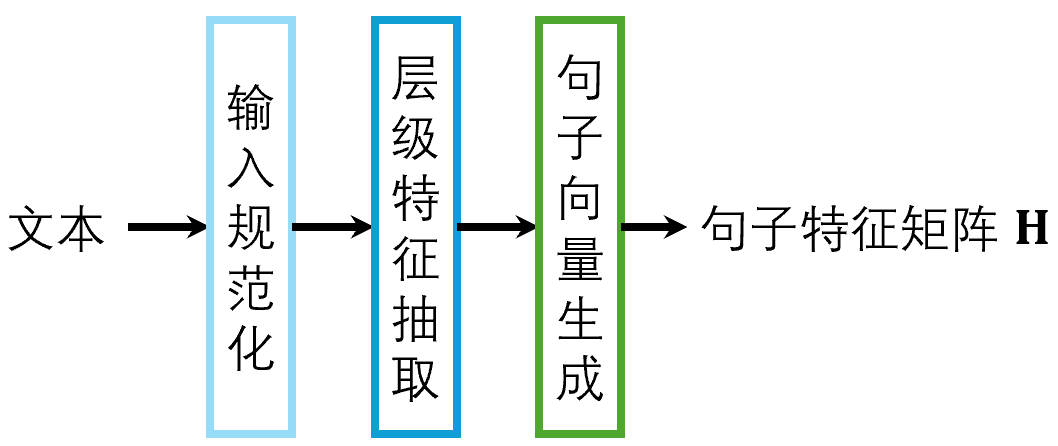
\includegraphics[width=0.6\textwidth]{figures/feature_extract.jpg}
    \caption{句子的特征提取}
    \label{fig:method-feature-extract}
\end{figure*}

特征提取模块中,单个句子$s_i$的编码主要分为以下三个阶段:

(1)阶段一:输入规范化

\textbf{分词与截断}:采用分词器对句子进行词切分后,生成对应token序列$[t_{i1}, t_{i2}, ..., t_{ik}]$(假设$s_i$分词后的token序列长度为$k$),然后对该序列执行动态填充(padding)与截断(truncation),确保最大序列长度不超过512。

\textbf{添加特殊标记}:在序列首尾分别添加 \texttt{[CLS]} 和 \texttt{[SEP]},形成规范化输入序列为 \( (\texttt{[CLS]}, t_{i1}, t_{i2}, \ldots, t_{ik}, \texttt{[SEP]}) \),其中 \(\texttt{[CLS]} \) 标记的隐藏状态作为全局语义表征将用于后续句子表征向量的生成。

(2)阶段二:层级特征抽取

\textbf{嵌入层映射}:通过三元嵌入组合(Token + Position + Segment)将离散输入映射为 768 维稠密向量。对$s_i$中每个位置 $j$ 的嵌入计算为:
\begin{equation}
    \textbf{E}_j = \textbf{E}_{token,j} + \textbf{E}_{pos,j} + \textbf{E}_{seg,j}, \quad j \in [1,k]
\end{equation}
其中,$\textbf{E}_{token,j}$ 表示词嵌入,$\textbf{E}_{pos,j}$ 表示绝对位置嵌入,$\textbf{E}_{seg,j}$ 表示段落嵌入。最终得到第 $i$ 个句子的嵌入矩阵$\textbf{E} \in \mathbb{R}^{k \times 768}$ 包含所有位置的联合表示,包括特殊标记\texttt{[CLS]} 和\texttt{[SEP]}。

\textbf{深度编码传播}:通过12层双向Transformer编码器对$s_i$的嵌入进行独立处理,逐步融入更深层次的语义。编码过程中第$l$层输出为:
\begin{equation}
    \textbf{H}^{(l)} = \text{LayerNorm}\left(\textbf{H}^{(l-1)} + \text{Attention}_\text{Transformer}(\textbf{H}^{(l-1)})\right)
\end{equation}
其中第一层的输入向量$\textbf{H}^0=\textbf{E}$,经过12层编码后最终得到句子$s_i$的上下文感知表示$\textbf{H}^{\text{final}} \in \mathbb{R}^{k \times 768}$。

(3)阶段三:句子向量生成

得到句子的层级特征之后,不同于直接提取首标记隐藏状态作为全局表征的做法,本模型采用混合池化策略提取每个句子的多模式特征以保留原始句子的细粒度语义。

具体来说,对于句子$s_i$,混合池化步骤需要分别计算其 $\texttt{[CLS]}$ 全局表征$\textbf{h}^\texttt{[CLS]}$($\texttt{[CLS]}$ 标记池化)、序列有效token部分的平均向量$\textbf{h}^\text{mean}$(均值池化)以及序列有效token部分沿特征维度的最大值$\textbf{h}^\text{max}$(最大池化),具体计算方式如下:
\begin{equation}
    \textbf{h}^\texttt{[CLS]} = \textbf{H}^{\text{final}}[0, :] \in \mathbb{R}^{768}
\end{equation}
\begin{equation}
    \textbf{h}^{\text{mean}} = \frac{1}{k} \sum_{j=1}^{k} \textbf{H}^{\text{final}}[j, :]
\end{equation}
\begin{equation}
    \textbf{h}^{\text{max}} = \max_{1 \leq j \leq k} (\textbf{H}^{\text{final}}[j, :])
\end{equation}

混合池化操作结束后还需要对语义向量与对应的混合池化表征进行投影降维。通过可学习的投影矩阵$\textbf{W}_p$将高维度混合特征映射至目标维度,最终得到单个句子的编码向量。整体计算流程如式\ref{sentence_embedding_generate}所示:
\begin{equation}\label{sentence_embedding_generate}
    \textbf{h} = \textbf{W}_p[\textbf{h}^\texttt{[CLS]}; \textbf{h}^{\text{mean}}; \textbf{h}^{\text{max}}] \in \mathbb{R}^d
\end{equation}
其中 $\textbf{W}_p \in \mathbb{R}^{d \times d_\text{hidden}}$ 为可学习参数矩阵,$d$ 为输出维度(默认768),$d_\text{hidden}$为投影维度。

\subsubsection{句子间注意力权重计算}

在 Transformer 中,定义注意力函数为输入为查询和一组键值,然后进行输出的函数,在此之中查询(Query, Q)、键(Key, K)、值(Value, V)和输出都是向量。在注意力函数中,简单地讲,输出实质上是值的加权和。此其中对于每个值的权重由权重相应的键以及查询计算得出。

本文中设计的句子间注意力权重计算过程参考了 Transformer 中的注意力机制 \cite{transformer} 并加以修改,其核心思想是通过计算查询与键之间的相似度来确定值的权重。在本文中,句子间注意力权重计算采用了单层基于稀疏掩码缩放点积注意力的多头注意力机制。以下是对这两种机制的详细介绍。

(1) 稀疏掩码缩放点积注意力

在 Transformer 论文中所采用的注意力机制为缩放点积注意力。该机制的输入由查询、键和值组成,其中查询和键的维度均为 \(d_k\),而值的维度为 \(d_v\)。在句子间注意力权重计算中,输入的查询、键和值都为句子特征矩阵 \(\textbf{H}\)。此外,基于语言学中句子关联性的距离衰减特性(即相邻句子通常具有更强的语义关联),本文在注意力机制中引入了稀疏掩码策略,具体通过设置距离阈值(distance threshold=3)来屏蔽远距离句子间的注意力交互。这种设计实现了两个关键优势:(1)符合文本的局部连贯性原理;(2)显著降低了长文档处理时的计算复杂度。

\begin{figure}[htbp]
	\centering
	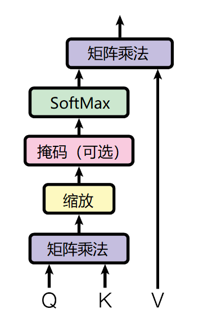
\includegraphics[scale = 0.4]{figures/DotAtt}
	\caption{稀疏掩码缩放点积注意力}
	\label{fig:DotAtt}
\end{figure}

在本文应用的稀疏掩码缩放点积注意力中,首先将句子特征矩阵 \( \textbf{H} \) 通过三个各不相同的线性层,再计算两个句子特征矩阵的乘积,并随后将矩阵乘法的结果除以系数 \(\sqrt{d_k}\)。再使用稀疏掩码遮掩距离过远的句子之间的注意力,接着,通过 softmax 函数后再与句子特征矩阵 \( \textbf{H} \) 做矩阵乘法,求出单次稀疏掩码缩放点积注意力。具体的过程如图 \ref{fig:DotAtt} 所示。

稀疏掩码缩放点积注意力函数的输出可以表示为:
\begin{equation}
\text{Attention}_\text{sparse}(\textbf{H}) = \text{SoftMax} \left( \frac{(\textbf{HW}^Q)(\textbf{HW}^K)^T}{\sqrt{d_k}} \odot \textbf{M} \right) (\textbf{HW}^V)
\label{eq3.1}
\end{equation}
其中,\(\textbf{M}\) 为稀疏掩码矩阵,\(\odot\) 表示遮蔽掩码操作。\(\textbf{W}^Q \in \mathbb{R}^{d_{\text{model}} \times d_k}\)、\(\textbf{W}^K \in \mathbb{R}^{d_{\text{model}} \times d_k}\)、\(\textbf{W}^V \in \mathbb{R}^{d_{\text{model}} \times d_v}\) 分别为图 \ref{fig:DotAtt} 中线性层 Q、线性层 K 和线性层 V 的权重矩阵。

(2) 多头注意力

本文为防止可能产生的模型性能下降问题,因此没有将键、值和查询的维度统一设定为 \(d_{\text{model}}\) 。在线性层中将查询、键和值分别投影为 \(d_k\)、\(d_k\) 和 \(d_v\) 维度。在此基础上,经过一系列操作生成 \(d_v\) 维的输出值。随后,将这些 \(d_v\) 维的输出值进行连接,并再次进行线性投影,以生成最终输出。具体过程如图 \ref{fig:MultiheadAtt} 所示。

\begin{figure}[htbp]
	\centering
	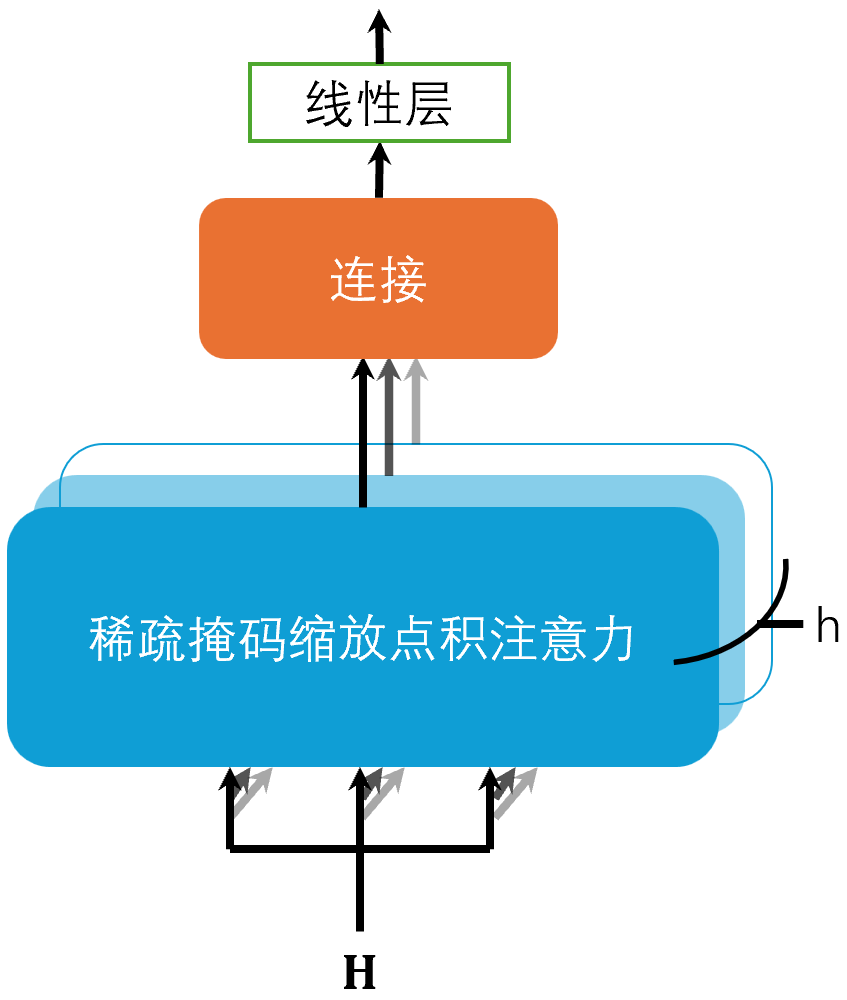
\includegraphics[scale = 0.4]{figures/MultiheadAtt}
	\caption{多头注意力 \cite{transformer}}
	\label{fig:MultiheadAtt}
\end{figure}

相较于单注意力头会导致信息的平均化,不同位置的信息可以被多头注意力同时关注。多头注意力机制的输出可以表示为:
\begin{equation}
\textbf{W} = \text{Attention}(\textbf{H}) = \text{Concat} \left(\text{Attention}_\text{sparse-1}(\textbf{H}), ..., \text{Attention}_\text{sparse-h}(\textbf{H}) \right)W^O
\label{eq3.2}
\end{equation}
在上述公式中,投影操作涉及的参数矩阵包括 \(\textbf{W}^Q \in \mathbb{R}^{d_{\text{model}} \times d_k}\)、\(\textbf{W}^K \in \mathbb{R}^{d_{\text{model}} \times d_k}\)、\(\textbf{W}^V \in \mathbb{R}^{d_{\text{model}} \times d_v}\) 以及 \(\textbf{W}^O \in \mathbb{R}^{hd_v \times d_{\text{model}}}\)。

在句子间注意力权重计算中,本文采用了 \(h = 8\) 个注意力头。\(d_k = d_v = d_{\text{model}} / h = 64\) 的维度赋予给了每一个注意力头。注意到,由于 \(d_k, d_v, d_{\text{model}} \) 被放缩,因此整体计算成本与具有全维度的单头注意力等价。

\subsection{句子检测}

句子检测模块旨在对单个句子的来源进行判断,具体框架如图\ref{fig:sentence-classifier}所示,主要包含三个组成部分,分别是:词嵌入层,特征提取器,以及分类器。

\begin{figure*}[htbp]
    \centering
    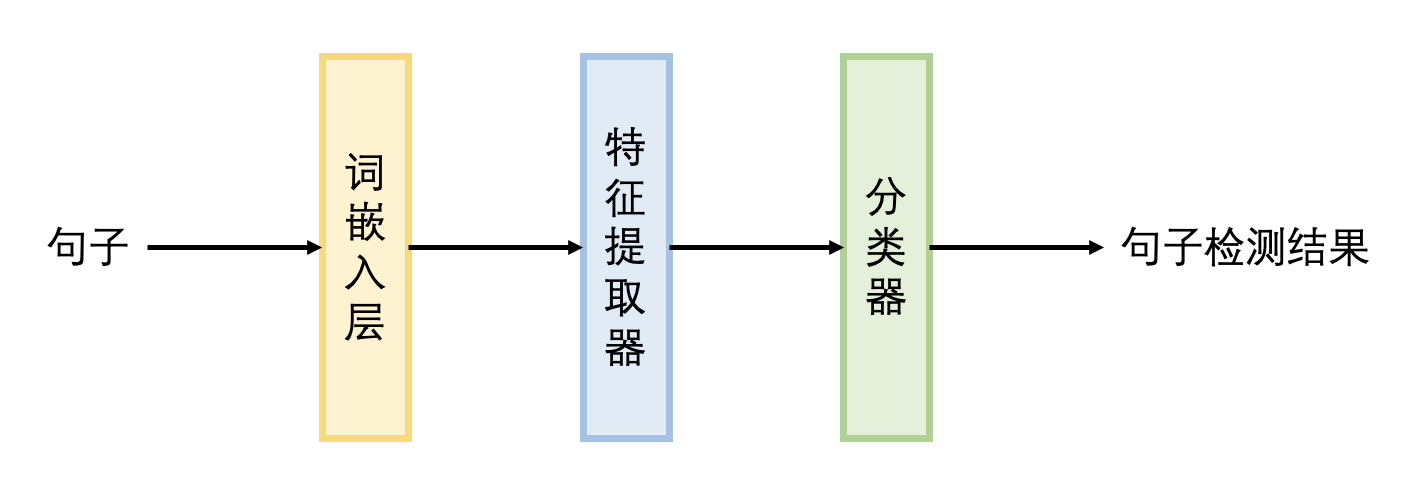
\includegraphics[width=0.9\textwidth]{figures/sentence-classifier.png}
    \caption{句子检测模块框架图}
    \label{fig:sentence-classifier}
\end{figure*}

给定一个待检测句子$S$,首先利用分词器对其进行词元化处理,表示为由$n$个词元$t_{i}$顺序排列组成的序列$[t_{1}, t_{2}, \ldots, t_{n}]$。本文采用的是DeBERTa-V3-Large对应的分词器,它会在每个序列前面自动添加一个$[\mathrm{CLS}]$词元,用于整合整个序列语义,因此处理后的句子$S=[t_{0}, t_{1}, t_{2}, \ldots, t_{n}]$, $t_{0}$对应$[\mathrm{CLS}]$词元。

将待检测句子$S$处理完毕后,利用句子检测模块对其进行检测。首先将其输入到词嵌入层$\mathrm{Embedding}(\cdot)$,将离散的词元转变为稠密的向量表示,便于后续利用神经网络进行特征提取,得到每个词元$t_{i}$对应的词嵌入表示$\mathbf{e}_{i}$:
\begin{equation}
    [\mathbf{e}_{0}, \mathbf{e}_{1}, \ldots, \mathbf{e}_{n}]=\mathrm{Embedding}([t_{0}, t_{1}, \ldots, t_{n}])
\end{equation}

为了挖掘句子的深层语义特征,利用预训练DeBERTa-V3-Large模型作为特征提取器,对句子进行特征表征,得到每个词元对应的隐层表征向量$\mathbf{h}_{i}$:
\begin{equation}
    [\mathbf{h}_{0}, \mathbf{h}_{1}, \ldots, \mathbf{h}_{n}]=\mathrm{DeBERTa}([\mathbf{e}_{0}, \mathbf{e}_{1}, \ldots, \mathbf{e}_{n}])
\end{equation}

由于在DeBERTa-V3-Large模型预训练过程中,$[\mathrm{CLS}]$词元用于整合句子的全局语义信息,以往研究常常将其对应的隐层表征向量$\mathbf{h}_{0}$当做句子全局特征,用于下游的分类任务。本文沿用该方式,将$[\mathrm{CLS}]$词元对应的隐层向量$\mathbf{h}_{0}$作为特征传入分类器,对句子进行检测。分类器由线性层$\mathrm{Linear}(\cdot)$和$\mathrm{SoftMax}(\cdot)$组成:
\begin{equation}
    \mathbf{p}=\mathrm{SoftMax}(\mathrm{Linear}(\mathbf{h}_{0}))
\end{equation}
其中,$\mathbf{p}$为模型的预测概率分布。

训练阶段,模型采用交叉熵损失函数来计算模型预测结果和实际标签之间的差异。利用句子级检测数据对本模块进行调优,能够有效捕捉文本中的细微差异和潜在模式,实现准确和可靠的句子级检测,为后续文档级文本检测提供坚实基础。在后续的模型设计中,该模块所有参数被冻结,不再参与整体模型参数的更新,从而节约计算成本。即便如此,模型整体性能并未受到过多影响,仍能实现较高的文档级检测准确率。

\section{实验}
\label{sec:method-experiment}

本文设计了如下实验,基于在第 \ref{chap:TOSWT} 章中介绍的模型改写文本检测数据集微调 \ref{sec:method-pretrain-roberta} 节中提及的 RoBERTa-Base 和 RoBERTa-Large 以及在 \ref{sec:method-pretrain-deberta} 节中提及的 DeBERTa-V3-Base 和 DeBERTa-V3-Large 模型。以及在文档级微调实验中,使用 \ref{sec:method-sent2arti} 中提及的基于句子级文本检测技术的文档级文本检测方法四种方法。微调后再调用模型在测试集上输出预测标签,最后使用四种指标准确率(Accuracy)、精确率(Precision)、召回率(Recall)和 F1 分数评估预测标签的水准,进而评定微调后的模型能力。

为满足细粒度的数据要求,分别使用文档级别和句子级别的数据分别微调上文提及的四个模型。这些预训练模型参数来源 URL 如表 \ref{tab:method-pretrain_model_url} 所示。

\begin{table*}[htbp]
\centering
\caption{预训练模型参数来源 URL} \label{tab:method-pretrain_model_url}
\begin{tabular}{ll}
\toprule
\textbf{模型}      & \textbf{来源 URL}                                                                 \\ \midrule
bge-base-en-v1.5 \cite{bge_embedding} & \url{https://huggingface.co/BAAI/bge-base-en-v1.5} \\ 
RoBERTa-Base \cite{liu_roberta_2019}     & \url{https://huggingface.co/FacebookAI/roberta-base}    \\
RoBERTa-Large \cite{liu_roberta_2019}   & \url{https://huggingface.co/FacebookAI/roberta-large}   \\
DeBERTa-V3-Base \cite{he2023debertav3improvingdebertausing}  & \url{https://huggingface.co/microsoft/deberta-v3-base}  \\
DeBERTa-V3-Large \cite{he2023debertav3improvingdebertausing} & \url{https://huggingface.co/microsoft/deberta-v3-large} \\ \bottomrule
\end{tabular}
\end{table*}

% 除了该对比实验外,我们还设计了消融实验,在 AES2 数据集评分基础上,进一步探索大语言模型改写文本的能力。有这样两个问题:原始文本对于大语言模型改写文本的影响有多大?大语言模型改写文本后,新文本的文本质量与原始文本质量一致性如何?为深入探索这两个问题,我们同样设计了两个额外的消融实验放置于 \ref{sec:method-experiment-analysis} 中。

\subsection{数据集设置}
\label{sec:method-experiment-dataset}

本实验中数据集采用在第 \ref{chap:TOSWT} 章中介绍的模型改写文本检测数据集。数据集示例如表 \ref{tab:TOSWT-eg} 所示,受单页篇幅所限,这里选取了一个包含两个句子的数据示例,该示例数据评分在其原始 AES2 数据集中被评定为 2 分。

\begin{table*}[htbp]
\BITSetup{ misc / tabularFontSize = 6}
\centering
\caption{模型改写文本检测数据集数据示例} \label{tab:TOSWT-eg}
\begin{tabular}{lp{12cm}}
\toprule
\multicolumn{1}{c}{\textbf{模型}} & \multicolumn{1}{c}{\textbf{文本}}  \\ \midrule
AES2 \cite{learning-agency-lab-automated-essay-scoring-2}                            & Luke think you should join the   seagoing cowboys program because you can travel all around and see some   pretty nice things like Luke it said in the passage that you take nine trips   to things like Greece,China,you will past the Atlantic Ocean and also you can   make the world a better place and you can be a hero for being nice. Also so if you want to you can help out animals in the passage it said, the   animals had to drink two or three times a day also a way you can help you   could clean the stalls on the ship and they will give you jobs and other   stuff and so you won't think it is boring you can have fun onboard to they   got a lot of things like baseball,and volleyball and the house it is   table-tennis tournaments,fencing,boxing,reading,whittling,and the games make   time go fast and that's why I think you should join the seagoing Cowboys   program. \\ \midrule
GPT3.5 \cite{chatgpt}                         & Luke thinks you should   join the Seagoing Cowboys program because you can travel all around and see   some pretty nice things. Like Luke said in the passage, you can take nine   trips to places like Greece and China. You will cross the Atlantic Ocean, and   you can make the world a better place by being nice and becoming a   hero. Also, if you want to, you can help out animals. In the passage, it said   that the animals had to drink two or three times a day. Another way you can   help is by cleaning the stalls on the ship. They will give you jobs and other   stuff. And so you won't think it's boring, you can have fun onboard too. They   have a lot of things like baseball, volleyball, table-tennis tournaments,   fencing, boxing, reading, and whittling. The games make time go fast, and   that's why I think you should join the Seagoing Cowboys program.   \\ \midrule
GPT4o \cite{gpt4o}                          & Luke believes you should join the seagoing   cowboys program because it allows you to travel extensively and see beautiful   places; as mentioned in the passage, you can undertake trips to destinations   like Greece and China, cross the Atlantic Ocean, and make the world a better   place while becoming a hero by being kind. Additionally, if you wish, you can assist with caring for animals; the   passage noted that the animals need to drink two or three times a day, and   one of the ways you can contribute is by cleaning the stalls on the ship,   where they will provide you with various tasks to keep you engaged, along   with fun activities such as baseball and volleyball, as well as other   pastimes like table tennis tournaments, fencing, boxing, reading, whittling,   which help make the time fly by-these are the reasons I think you should join   the seagoing Cowboys program. \\ \midrule
Gemini \cite{geminiteam2024geminifamilyhighlycapable}                         & Luke believes you should join   the Seagoing Cowboys program because it offers the opportunity to travel   extensively and witness beautiful sights, as he mentioned in the passage that   participants take nine trips to destinations like Greece and China, traverse   the Atlantic Ocean, and contribute to making the world a better place,   potentially becoming a hero through acts of kindness. Additionally, if you're interested, you can assist animals, as the passage   mentioned that they need to drink two or three times daily; you could also   help by cleaning stalls on the ship, and they'll provide you with various   tasks and activities to keep you engaged and prevent boredom, as there are   plenty of recreational options onboard, including baseball, volleyball, table   tennis tournaments, fencing, boxing, reading, whittling, all of which help   pass the time quickly, and that's why I believe you should consider joining   the Seagoing Cowboys program. \\ \midrule
Qwen \cite{qwen2025qwen25technicalreport}                           & Luke believes you should join   the seagoing cowboys program because it offers opportunities to travel   extensively and see beautiful places, such as Greece and China, as mentioned   in the passage. You will cross the Atlantic Ocean and contribute to making the   world a better place, thereby becoming a hero by being kind and   helpful. Additionally, if you wish, you can assist animals, as the passage notes   they need to drink two or three times a day. You could help by cleaning the   ship's stalls and taking on various jobs, ensuring the journey is enjoyable.   Onboard activities like baseball, volleyball, table tennis tournaments,   fencing, boxing, reading, and whittling make time pass quickly, which is why   I think you should join the seagoing cowboys program. \\ \midrule
DeepSeek \cite{deepseekai2024deepseekv3technicalreport}                       & Luke believes you should join   the seagoing cowboys program because it offers the opportunity to travel   extensively and witness beautiful sights, such as Greece and China, while   crossing the Atlantic Ocean, and it allows you to make the world a better place   and become a hero through kindness. Additionally, if you wish, you can assist animals, as mentioned in the   passage, which require drinking two or three times daily, and you can   contribute by cleaning the stalls on the ship, where they provide jobs and   other activities to ensure it's not boring; you can also enjoy onboard   entertainment like baseball, volleyball, table-tennis tournaments, fencing,   boxing, reading, whittling, and games that make time pass quickly, which is   why I recommend joining the seagoing cowboys program. \\ \bottomrule
\end{tabular}
\end{table*}

对于文档级数据,我们将模型改写文本检测数据集分割为训练集、验证集与测试集。这三个被分割后的小数据集在大数据集随机打乱后分别按照文档的个数以 $7:1:2$ 的比例分割出来。待微调的模型在训练集上微调过后,该模型在验证集上得到初步的模型效果,随后选取损失函数最低的模型在测试集上测试,进而得到最终的效果。

而句子级数据中关于数据集的分割步骤也与文档级数据的分割步骤类似。只不过第一步需要先将所有句子分割出来,单独打上标签,按照句子的个数随机打乱顺序后再以 $7:1:2$ 的比例分割为训练集、验证集和测试集。

对于词元个数过长的数据用例,我们将长度大于 512 后面的部分完全截断。不过,这一步是在词元化(tokenizer)的过程中处理的。

\subsection{实验参数设置}
\label{sec:method-experiment-parameter}

% 本章节所有实验均在配备NVIDIA TITAN RTX显卡(24GB显存)的高性能计算服务器上完成,服务器运行Ubuntu Linux 22.04 LTS操作系统。为保障实验环境的可重复性,我们详细记录了硬件配置和软件环境参数:服务器基础配置信息如表 \ref{tab:os-env} 所示;显卡详细规格参数(包括CUDA版本、驱动版本等)如表 \ref{tab:gpu-env} 所列;实验代码基于Anaconda搭建的Python 3.12.8虚拟环境执行,其中关键依赖库(如PyTorch、Transformers等)的具体版本信息详见表 \ref{tab:python-env}。所有实验环境参数均经过严格测试验证,确保实验结果的可靠性和可复现性。

所有实验均运行于 Ubuntu Linux 22.04 服务器上。详细实验操作系统环境如表 \ref{tab:os-env} 所示。

\begin{table*}[h]
\centering
\caption{实验操作系统环境} \label{tab:os-env}
\begin{tabular}{ll}
\toprule
\textbf{字段}    & \textbf{值}                               \\ \midrule
内核版本           & 6.8.0-49-generic                         \\
构建环境           & buildd@lcy02-amd64-103                   \\
架构             & x86\_64 (64位)                             \\
编译器            & x86\_64-linux-gnu-gcc-12                  \\
编译器版本          & 12.3.0                                   \\
编译器来源          & Ubuntu 12.3.0-1ubuntu1\textasciitilde22.04             \\
链接器   (GNU ld) & GNU Binutils for Ubuntu 2.38             \\
构建编号           & \#49\textasciitilde22.04.1-Ubuntu                       \\
构建类型           & SMP (对称多处理) + PREEMPT\_DYNAMIC(动态抢占模式) \\
构建时间           & Wed Nov 6 17:42:15 UTC 2024              \\
发行版基础          & Ubuntu 22.04.1 LTS                       \\ \bottomrule
\end{tabular}
\end{table*}

本章节全部实验均在拥有 24GB 显存容量的 NVIDIA TITAN RTX 显卡上完成,该显卡详细环境如表 \ref{tab:gpu-env} 所示。

\begin{table*}[h]
\centering
\caption{实验显卡环境} \label{tab:gpu-env}
\begin{tabular}{ll}
\toprule
\textbf{字段} & \textbf{值}           \\ \midrule
GPU   型号    & NVIDIA TITAN RTX     \\
GPU   架构    & Turning              \\
显存容量        & 24GB                 \\
TDP   (功耗)  & 320W                 \\
驱动版本        & NVIDIA-SMI 560.35.03 \\
CUDA   版本   & 12.6                 \\ \bottomrule
\end{tabular}
\end{table*}

本章节实验在实现上基于 Anaconda 库中搭建的 Conda 虚拟环境运行 Python 代码,Python 环境中部分重要包版本号如表 \ref{tab:python-env} 所示。

\begin{table*}[htbp]
\BITSetup{ misc / tabularFontSize = 6}
\centering
\caption{实验 Python 环境部分重要包版本} \label{tab:python-env}
\begin{tabular}{cll}
\toprule
\textbf{分类}                  & \textbf{字段}       & \textbf{版本号} \\ \midrule
\multirow{28}{*}{基础}         & conda             & 24.9.2       \\
                             & Python            & 3.12.8       \\
                             & GCC               & 11.2.0       \\
                             & cuda-cudart       & 11.8.89      \\
                             & cuda-cupti        & 11.8.87      \\
                             & cuda-libraries    & 11.8.0       \\
                             & cuda-nvrtc        & 11.8.89      \\
                             & cuda-nvtx         & 11.8.86      \\
                             & cuda-runtime      & 11.8.0       \\
                             & cuda-version      & 12.6         \\
                             & ipython           & 8.30.0       \\
                             & json5             & 0.9.25       \\
                             & matplotlib        & 3.9.2        \\
                             & matplotlib-base   & 3.9.2        \\
                             & matplotlib-inline & 0.1.6        \\
                             & nltk              & 3.9.1        \\
                             & numpy             & 2.0.1        \\
                             & openai            & 1.52.1       \\
                             & pandas            & 2.2.3        \\
                             & pillow            & 11.0.0       \\
                             & pip               & 24.2         \\
                             & regex             & 2024.11.6    \\
                             & sentencepiece     & 0.2.0        \\
                             & scikit-learn      & 1.6.0        \\
                             & scipy             & 1.14.1       \\
                             & tensorboard       & 2.17.0       \\
                             & xlsxwriter        & 3.1.1        \\
                             & yaml              & 0.2.5        \\ \midrule
\multirow{6}{*}{Torch}       & pytorch           & 2.5.1        \\
                             & pytorch-cuda      & 11.8         \\
                             & pytorch-mutex     & 1.0          \\
                             & torchaudio        & 2.5.1        \\
                             & torchtriton       & 3.1.0        \\
                             & torchvision       & 0.20.1       \\ \midrule
\multirow{5}{*}{HuggingFace} & accelerate        & 1.2.1        \\
                             & datasets          & 3.2.0        \\
                             & huggingface-hub   & 0.27.0       \\
                             & tokenizers        & 0.21.0       \\
                             & transformers      & 4.47.1       \\ \bottomrule
\end{tabular}
\end{table*}

在基础的文档级和句子级的数据实验中,我们使用 DeBERTa 和 RoBERTa 作为实验用的模型并微调了四种模型:RoBERTa-Base、RoBERTa-Large、DeBERTa-Base 和 DeBERTa-Large,可变超参数包括批大小(batch size, BS)、学习率(learning rate, LR)、权重衰减系数(weight decay, WD)。在所有实验中,学习率均采用余弦退火衰减算法,并使用 AdamW 算法作为优化器。超参数详见表 \ref{tab:hyper-parameters},其中,在句子级实验中,大尺寸模型如 RoBERTa-Large 和 DeBERTa-V3-Large 的超参数均经过广泛地搜索长时间实验才找到可以使模型拟合于数据的一组超参数。DeBERTa-V3-Large 由于其总参数量较大,为防止超出显卡显存,因此批大小相较其他实验的 16 个为一批较小,设置为 4 个为一批。

\begin{table*}[htbp]
\centering
\caption{对比试验微调超参数列表}
\label{tab:hyper-parameters}
\begin{tabular}{c|l|ccc}
\toprule
                          & \textbf{模型}   & \textbf{批大小} & \textbf{初始学习率} & \textbf{权重衰减系数} \\ \midrule
\multirow{4}{*}{文档级}    & RoBERTa-Base \cite{liu_roberta_2019}     & 16                  & $10^{-5}$                & 0.01                  \\
                          & RoBERTa-Large \cite{liu_roberta_2019}    & 16                  & $10^{-5}$                & 0.01                  \\
                          & DeBERTa-V3-Base \cite{he2023debertav3improvingdebertausing}  & 16                  & $10^{-5}$                & 0.01                  \\
                          & DeBERTa-V3-Large \cite{he2023debertav3improvingdebertausing} & 4                   & $10^{-5}$                & 0.01                  \\ \midrule
\multirow{4}{*}{句子级}    & RoBERTa-Base \cite{liu_roberta_2019}     & 16                  & $10^{-5}$                & 0.01                  \\
                          & RoBERTa-Large \cite{liu_roberta_2019}    & 16                  & $10^{-6}$               & 0.0001                \\
                          & DeBERTa-V3-Base \cite{he2023debertav3improvingdebertausing}  & 16                  & $10^{-5}$                & 0.01                  \\
                          & DeBERTa-V3-Large \cite{he2023debertav3improvingdebertausing} & 4                   & $10^{-6}$               & 0.001                 \\ \midrule
句子级推测文档级 & 句子深度贡献度加权 & 8 & $10^{-6}$ & 0.001 \\ \bottomrule
\end{tabular}
\end{table*}

\subsubsection{交叉熵损失函数}

交叉熵函数 \cite{CrossEntropy} 是信息论和机器学习领域中的一个基本概念,主要用于量化两个概率分布之间的差异。其数学表达式为:对于真实分布 \( P \) 和预测分布 \( Q \),交叉熵 \( H(P, Q) \) 定义为:
\(
H(P, Q) = -\sum_x P(x) \log Q(x)
\)
。交叉熵反映了使用分布 \( Q \) 编码从分布 \( P \) 中抽取事件所需的平均比特数。当 \( Q \) 越接近于 \( P \) 时,交叉熵的值将趋向于减少。

在机器学习的应用中,交叉熵常常被用作分类任务的损失函数。例如,在本文讨论的六分类问题中,针对 \( m \) 个样本,该损失函数可以表示为:
\begin{align}
    L=-\frac{1}{m}\sum_{i=1}^m \sum_{j=1}^6 t_{ij}\log(y_{ij})
\end{align}
其中,\( t_{ij} \) 表示真实标签(采用 one-hot 编码),而 \( y_{ij} \) 则是模型的预测概率。这种损失函数设计能够有效地惩罚预测错误,尤其是在与 Softmax 或 Sigmoid 激活函数结合使用时,能够高效地计算梯度,并避免均方误差在学习过程中导致的学习速率下降问题。

交叉熵与信息熵及 KL 散度之间存在密切的关系。信息熵 \( H(P) \) 代表分布 \( P \) 的最佳编码长度,而交叉熵 \( H(P, Q) \) 则是使用分布 \( Q \) 编码 \( P \) 的代价。两者之间的差值即为 KL 散度,反映了两个分布之间的差异。在实际应用中,需要注意数值的稳定性,例如,通过对 \( Q(x) \) 进行裁剪以防止出现 \( \log(0) \) 的错误。

将交叉熵函数作为损失函数的优点在于其理论基础的严谨性与实践中的高效性。例如,在图像分类任务中,交叉熵直接优化预测概率与真实标签之间的匹配程度;而在本文所涉及的自然语言处理领域,它用于评估生成文本的概率分布的质量。

\subsubsection{AdamW 优化器}

AdamW 优化器 \cite{AdamW} 是对原始 Adam 优化器 \cite{Adam} 的一种重要改进,其算法流程如算法 \ref{algo:AdamW} 所示。该算法由 Ilya Loshchilov 和 Frank Hutter 于 2017 年提出,旨在解决传统 Adam 优化器在权重衰减(Weight Decay)处理方面的不足。在原始的 Adam 优化器中,权重衰减是通过将衰减项直接纳入梯度更新中来实现的。这种方法使得权重衰减的效果受到自适应学习率的影响,进而可能削弱正则化的有效性。相比之下,AdamW 优化器通过将权重衰减与梯度更新过程解耦,使其独立于梯度更新步骤,从而能够更准确地实现正则化效果。这一改进不仅提高了优化过程的稳定性,也增强了模型的泛化能力。

\begin{algorithm}[htb]
\caption{AdamW 优化算法} \label{algo:AdamW}
\begin{algorithmic}[1]
    \Require 学习率 $\psi(\text{lr})$, $\beta_1$, $\beta_2$ (betas), 初始参数 $\theta_0$ (params), 目标函数 $f(\theta)$ (objective), $\epsilon$, 权重衰减 $\chi$, amsgrad, maximize
    \Ensure $\theta_t$
    
    \State 初始化: $m_0 \leftarrow 0$ (一阶矩), $v_0 \leftarrow 0$ (二阶矩), $\widehat{v_0}^{max} \leftarrow 0$
    \For {$t = 1$ to $\ldots$}
        \If{maximize}
            \State $g_t \leftarrow - \nabla_\theta f_t(\theta_{t-1})$
        \Else
            \State $g_t \leftarrow \nabla_\theta f_t(\theta_{t-1})$
        \EndIf
        
        \State $\theta_t \leftarrow \theta_{t-1} - \psi \chi \theta_{t-1}$ \Comment{权重衰减}
        
        \State $m_t \leftarrow \beta_1 m_{t-1} + (1 - \beta_1) g_t$ \Comment{更新一阶矩}
        \State $v_t \leftarrow \beta_2 v_{t-1} + (1 - \beta_2) g_t^2$ \Comment{更新二阶矩}
        
        \State $\widehat{m_t} \leftarrow m_t / (1 - \beta_1^t)$ \Comment{偏差修正}
        \State $\widehat{v_t} \leftarrow v_t / (1 - \beta_2^t)$
        
        \If{amsgrad}
            \State $\widehat{v_t}^{max} \leftarrow \max(\widehat{v_{t-1}}^{\text{max}}, \widehat{v_t})$
            \State $\theta_t \leftarrow \theta_t - \psi \widehat{m}_t / (\sqrt{\widehat{v_t}^{\text{max}}} + \epsilon)$
        \Else
            \State $\theta_t \leftarrow \theta_t - \psi \widehat{m_t} / (\sqrt{\widehat{v_t}} + \epsilon)$
        \EndIf
    \EndFor
\end{algorithmic}
\end{algorithm}

AdamW 优化器的核心理念在于保留 Adam 优化器所具备的自适应学习率和动量机制,同时对权重衰减的处理方式进行改进。具体而言,AdamW 在参数更新过程中将权重衰减项独立于梯度计算,直接对参数施加衰减。这一方法显著增强了权重衰减的稳定性,有效防止了模型的过拟合现象,并提升了其泛化能力。实验结果表明,AdamW 在多种深度学习任务中均优于传统的 Adam 优化器,尤其在需要强正则化的情境下表现尤为突出。

AdamW 的优势体现在多个方面:首先,它提供了更为有效的正则化机制,从而更好地控制模型的复杂性;其次,在训练深度神经网络时展现出更为稳定的收敛性;最后,它适用于需要长时间训练的任务,如大语言模型(LLM)的预训练。然而,AdamW 也存在一些不足之处,例如对学习率和权重衰减系数的选择较为敏感,这要求进行更多的超参数调节,尤其在处理句子级别较大的模型时,调参工作显得尤为繁琐。

在实际应用中,AdamW 已成为多个深度学习框架(如 PyTorch)的默认优化器之一,特别适合于处理高维参数空间和复杂模型结构。其改进设计不仅保持了 Adam 的高效性,还进一步提升了模型的泛化性能,使其成为现代深度学习训练中的一项重要工具。

\subsubsection{余弦退火调度器}

余弦退火是一种在深度学习领域广泛应用的学习率调度策略,其核心理念是通过余弦函数的动态调整来优化模型的训练过程。该方法最早由 Ilya Loshchilov 和 Frank Hutter 在 2016 年提出的 SGDR 方法 \cite{SGDR} 中引入,随后迅速成为深度学习中的一项重要技术。余弦退火的名称源于其数学实现方式——学习率按照余弦函数曲线从初始值平滑下降至最小值,类似于金属加工中的退火过程,即先进行高温加热,随后缓慢冷却。

从数学原理的角度来看,余弦退火的公式为:
\begin{align}
\eta_t = \eta_{min} + \frac{1}{2}(\eta_{max} - \eta_{min})(1 + \cos(\frac{T_{cur}}{T_i}\pi))
\end{align}
其中,\(\eta_{max}\) 和 \(\eta_{min}\) 分别表示学习率的上限和下限,\(T_{cur}\) 是当前的训练步数,而 \(T_i\) 是总的训练步数。这一设计使得学习率在训练初期保持较高的值,以加速收敛,随后逐渐减小,从而便于模型对参数进行精细调整。与传统的阶梯式衰减或线性衰减方法相比,余弦退火提供了更为平滑的过渡,避免了学习率突变所引发的训练不稳定性。

在实际应用中,余弦退火展现出多重优势。首先,其周期性调整特性有助于模型跳出局部最优解,这对于处理多峰损失函数尤为有效。其次,该方法显著减少了人工调参的需求,通过预设的数学规律自动调整学习率,使其适用于各种复杂模型和大规模数据集。实验结果表明,在图像分类、自然语言处理等任务中,采用余弦退火策略的模型通常能实现更快的收敛速度和更优的泛化性能。例如,在 ImageNet 竞赛中,使用该策略的 ResNet 模型表现出了显著的性能提升。

\subsubsection{权重衰减算法}

权重衰减是一种在深度学习领域广泛应用的正则化技术,主要目的是防止模型出现过拟合现象。其基本原理是通过在损失函数中引入一个与权重参数的平方和成正比的惩罚项(即 \( L_2 \) 范数),以约束模型参数的大小。具体的数学表达式为:
\begin{align}
L' = L + \lambda \sum \theta_i^2
\end{align}
在此公式中,\( L \) 表示原始损失函数,\(\theta\) 是模型的权重,而 \(\lambda\) 是正则化系数,用于控制惩罚的强度。这样的设计使得模型在训练过程中更倾向于学习较小的权重值,从而降低模型的复杂度,避免对训练数据中噪声的过度敏感。

从实现机制的角度来看,权重衰减在梯度下降过程中直接影响参数的更新。以随机梯度下降为例,这一操作可以视为在每次迭代中对权重施加线性衰减,因此被称为“权重衰减”。需要指出的是,权重衰减通常不适用于偏置项,因为偏置主要负责输出的平移,对模型复杂性的影响相对较小。

权重衰减的作用机制可以从多个方面进行解释。首先,较小的权重使得模型对输入变化更加鲁棒,从而减少对噪声特征的依赖;其次,通过抑制特征之间的共线性,避免模型对某些特定特征组合的过度依赖;最后,它能够有效防止梯度爆炸问题,从而提升训练的稳定性。实验结果表明,在像 ImageNet 这样的大型数据集上,合理设置 \(\lambda\) 可以使测试误差降低 10\% 至 20\%。

在实际应用中,权重衰减常常与其他技术(如 Dropout 和批量归一化)结合使用。超参数 \(\lambda\) 的选择通常需要通过多次验证来确定,典型取值范围为 \(10^{-4}\) 到 \(10^{-2}\)。在本文中,我们经过多次测试确定了相应的权重衰减超参数。现代深度学习框架(如本文使用的 PyTorch)中内置了权重衰减功能,可以通过前述的 AdamW 优化器中的 weight\_decay 参数轻松启用。值得注意的是,尽管权重衰减与 \( L_2 \) 正则化在数学形式上相似,但其实现机制有所不同:前者直接修改优化过程,而后者则通过损失函数间接施加影响。

\subsection{评价指标}
\label{sec:method-experiment-metric}

本文共使用四种评价指标来评定,分别为\textbf{准确率}(Accuracy)、\textbf{精准率}(Precision)、\textbf{召回率}(Recall)和 \textbf{F1 分数}。这四种评价指标将在下面的小节中进行相应的介绍。由于模型改写文本检测本质上是多分类文本分类任务,因此后三者指标需要与二分类指标有相应变化。由于每个生成模型产生相同数量的文本,并且由于数据量对指标的影响最小,因此采用了对数据量敏感的宏观(macro)方法。

\subsubsection{准确率}

准确率(Accuracy)是机器学习中最基本且直观的分类评估指标,主要用于衡量模型整体预测的准确性。其核心定义为模型正确预测的样本数量占总样本数量的比例,数学表达式为:
\begin{align}
    Accuracy = \frac{TP+TN}{TP+TN+FP+FN}
\end{align}
在此公式中,\(TP\)(真正例)和 \(TN\)(真负例)分别表示正类和负类中预测正确的样本数量,而 \(FP\)(假正例)和 \(FN\)(假负例)则代表预测错误的样本数量。例如,在疾病诊断的场景中,如果模型成功识别了100名患者中的90名(包括健康和患病个体),则准确率为90\%,直观地反映了模型的综合判断能力。

\subsubsection{精准率}

精准率(Precision)是评估分类模型性能的重要指标之一,主要用于衡量模型预测为正类的样本中,实际为正类的比例。其数学定义为:
\begin{align}
    Precision = \frac{TP}{TP+FP}
\end{align}
在此公式中,\(TP\)(真正例)表示模型正确预测的正类样本数量,而 \(FP\)(假正例)则代表模型错误地将负类预测为正类的样本数量。该指标尤为关注模型预测为正类的可靠性。例如,在医疗诊断领域,高精准率意味着较少的健康患者被误诊为患病,从而避免不必要的治疗费用。

在本文的实验中,由于模型的文本改写检测本质上是一个多分类文本分类任务,因此精准率指标需要与二分类指标进行相应调整。考虑到每个生成模型产生相同数量的文本,并且数据量对指标的影响较小,因此采用了对数据量敏感的宏观(macro)方法进行评估。

\subsubsection{召回率}

召回率(Recall)是机器学习中用于评估分类模型性能的重要指标之一,主要用于衡量模型对正类样本的识别能力。其数学定义为:
\begin{align}
    Recall = \frac{TP}{TP+FN}
\end{align}
在此公式中,\(TP\)表示真正例,即模型正确预测的正类样本数量,而 \(FN\)则代表假负例,即实际为正类但被错误判定为负类的样本数量。该指标反映了所有真实正类样本中被模型成功识别的比例,因此也被称为“查全率”。在医疗诊断等高风险领域,高召回率意味着漏诊风险的降低。例如,如果癌症筛查模型的召回率达到90\%,则表明90\%的真实患者得到了正确检出。

在本文的实验中,由于模型的文本改写检测本质上属于多分类文本分类任务,因此召回率指标需要与二分类指标进行相应调整。考虑到每个生成模型产生相同数量的文本,并且数据量对指标的影响较小,因此采用了对数据量敏感的宏观(macro)方法进行评估。

\subsubsection{F1 分数}

F1分数是机器学习中评估分类模型性能的关键指标,它通过调和精确率(Precision)与召回率(Recall)来提供全面的性能评估。其计算公式为:
\begin{align}
    F1 = 2 \times \frac{Precision \times Recall}{Precision + Recall}
\end{align}
在此公式中,精确率用于衡量模型预测为正类的准确性(\(Precision = \frac{TP}{TP + FP}\)),而召回率则评估模型捕捉正类样本的能力(\(Recall = \frac{TP}{TP + FN}\))。这一设计使得F1分数对精确率与召回率赋予相同的重要性,任一指标的低下都会显著影响整体得分。

在本文的实验中,由于模型的文本改写检测本质上属于多分类文本分类任务,因此F1分数指标需要与二分类指标进行相应调整。考虑到每个生成模型产生相同数量的文本,并且数据量对指标的影响较小,因此采用了对数据量敏感的宏观(macro)方法进行评估。

\subsection{对比实验结果分析}
\label{sec:method-experiment-main}

本节通过两组对照实验系统评估了RoBERTa和DeBERTa模型在不同粒度文本理解任务中的表现。表 \ref{tab:document} 展示了文档级任务上的微调结果,其中DeBERTa-V3-Large以85.97\%的准确率和85.84\%的F1分数显著领先,验证了大规模预训练模型在处理长文本依赖关系时的优势。相比之下,表 \ref{tab:sentence} 揭示的句子级任务结果呈现出截然不同的特征:所有模型的绝对性能明显下降(最佳准确率仅49.61\%),且DeBERTa-V3-Base在精准率指标上意外超越其大型版本。这种差异凸显了文本处理粒度对模型性能的关键影响——文档级任务受益于丰富的上下文信息,而句子级任务则更依赖精准的局部语义理解。后续分析将深入探讨造成这种差异的内在机制,以及不同模型架构在两类任务中的适应性表现。

\subsubsection{文档级数据微调实验}

表 \ref{tab:document} 详细展示了RoBERTa和DeBERTa两个主流预训练语言模型家族在文档级自然语言处理任务上的微调性能对比结果。通过对准确率(Accuracy)、精准率(Precision)、召回率(Recall)和F1分数四个核心评估指标的全面分析,我们可以得出若干重要发现。

\begin{table*}[htbp]
\caption{RoBERTa 与 DeBERTa 模型在文档级数据上微调结果}
\centering
\begin{tabular}{l|cccc}
\toprule
\textbf{模型}& \textbf{准确率}   & \textbf{精准率}    & \textbf{召回率}    & \textbf{F1}   \\ \midrule
RoBERTa-Base \cite{liu_roberta_2019}  & 72.88          & 77.26          & 72.89          & 72.73          \\
RoBERTa-Large \cite{liu_roberta_2019} & 80.92          & 81.84          & 80.92          & 80.55          \\
DeBERTa-V3-Base \cite{he2023debertav3improvingdebertausing} & 79.85          & 81.44          & 79.85          & 79.81          \\
DeBERTa-V3-Large \cite{he2023debertav3improvingdebertausing} & \textbf{85.97} & \textbf{86.31} & \textbf{85.96} & \textbf{85.84} \\ \midrule
DeBERTa-V3-Large\cite{he2023debertav3improvingdebertausing}(Sentence)  & 78.11 & 80.63 & 78.11 & 77.87 \\
朴素加权 & 76.27 & 81.19 & 76.27 & 76.02 \\
长度加权 & 77.85 & 81.18 & 77.85 & 77.65 \\
句子深度贡献度加权 & \uline{78.26} & \uline{81.86} & \uline{78.26} & \uline{78.09} \\ \bottomrule
\end{tabular}
\label{tab:document}
\end{table*}

从整体性能趋势来看,所有评估指标都呈现出明显的层级结构:DeBERTa-V3-Large以显著优势领先,其准确率达到85.97\%,精准率86.31\%,召回率85.96\%,F1分数85.84\%,这四项指标均明显优于其他对比模型。这一结果验证了模型规模和架构改进的双重重要性。值得注意的是,DeBERTa-V3-Base(79.85\%准确率)与RoBERTa-Large(80.92\%准确率)的性能相当接近,这表明DeBERTa系列在基础模型规模下就能达到与更大规模RoBERTa模型相近的性能水平,充分体现了其架构设计的先进性。

深入分析模型架构的影响可以发现,DeBERTa系列采用的分离注意力机制和增强型掩码解码器带来了显著优势。特别是在精准率指标上,DeBERTa-V3-Base(81.44\%)已经超过了RoBERTa-Large(81.84\%),而DeBERTa-V3-Large更是将这一优势扩大到86.31\%。这表明DeBERTa的架构改进特别有利于提升模型预测的精确性,减少假阳性错误的发生。这一特性在需要高精度预测的应用场景(如医疗诊断或金融风险评估)中尤为重要。

从模型规模的角度观察,RoBERTa从Base到Large版本的性能提升幅度为8.04个百分点(准确率从72.88\%到80.92\%),而DeBERTa从Base到Large版本的提升幅度更大,达到6.12个百分点(从79.85\%到85.97\%)。虽然绝对提升值略低,但考虑到DeBERTa-Base的起点更高,这一相对提升仍然非常可观。这证实了增加模型参数规模对性能提升的持续有效性,同时也表明在优质架构设计的基础上,扩大模型规模能带来更显著的效果。

特别值得注意的是各模型在精准率和召回率之间的平衡关系。所有模型的精准率都略高于召回率,这种系统性差异可能反映了当前预训练语言模型在文档级任务中普遍存在的保守预测倾向。RoBERTa-Base的精准率(77.26\%)比召回率(72.89\%)高出4.37个百分点,这一差距在更大规模的模型中有所缩小,DeBERTa-V3-Large的精准率(86.31\%)仅比召回率(85.96\%)高出0.35个百分点。这表明随着模型规模和架构的优化,模型在保持高精确性的同时,也能更好地覆盖正类样本,实现更均衡的性能表现。

F1分数的变化趋势进一步验证了上述发现。作为精准率和召回率的调和平均数,F1分数综合反映了模型的整体分类性能。DeBERTa-V3-Large的F1分数达到85.84\%,比RoBERTa-Large的80.55\%高出5.29个百分点,这一提升幅度超过了准确率的提升(5.05个百分点),说明DeBERTa的优势在综合考虑精确性和全面性时更为明显。

在句子特征融合策略的比较中,本文提出的句子深度注意力机制以78.26\%的准确率表现最佳,比朴素加权方法提高了 1.99 个百分点,同时对比直接将文本输入句子级检测模型,完成了其指标的全面提升。长度加权方法也取得了不错的效果,F1值达到 77.65\%,说明文本长度这一特征确实能带来性能提升。然而,所有句子级特征融合策略的表现都明显低于完整文档级建模的DeBERTa-V3-Large模型,这突显了文档级整体建模的重要性。

从实际应用的角度来看,这些结果对模型选择具有重要指导意义。在计算资源允许的情况下,DeBERTa-V3-Large显然是首选方案;在资源受限时,DeBERTa-V3-Base能以较小的参数量达到与RoBERTa-Large相当的性能,是更经济高效的选择。此外,精准率普遍高于召回率的现象提示我们,在这些模型的工业部署中可能需要根据具体应用场景的需求,通过调整分类阈值来优化精确性或召回率。

这些实验结果也为未来研究指明了若干方向。首先,DeBERTa架构的成功验证了分离注意力机制在文档级任务中的有效性,值得进一步研究和扩展。其次,模型规模扩大带来的性能提升尚未达到平台期,暗示继续增大模型规模可能仍有潜力。最后,精准率和召回率之间的不平衡现象值得深入分析,可能需要设计专门的损失函数或训练策略来改善。

综上所述,表 \ref{tab:document} 通过系统的对比实验,不仅展示了不同预训练语言模型在文档级任务上的性能差异,更为模型架构设计、规模选择和实际应用提供了重要的实证依据。这些发现将有助于研究人员和工程师在文档级自然语言处理任务中做出更明智的模型选择和应用决策。

\subsubsection{句子级数据微调实验}

表 \ref{tab:sentence} 展示了RoBERTa和DeBERTa系列预训练语言模型在句子级自然语言处理任务上的微调性能对比。通过分析准确率(ACC)、精准率(P.)、召回率(R.)和F1分数四个关键评估指标,我们可以得出以下深入观察和结论。

\begin{table*}[htbp]
\caption{RoBERTa 和 DeBERTa 在句子级数据上微调结果}
\centering
\begin{tabular}{l|cccc}
\toprule
\textbf{模型}& \textbf{准确率}   & \textbf{精准率}    & \textbf{召回率}    & \textbf{F1}   \\ \midrule
RoBERTa-Base \cite{liu_roberta_2019}     & 45.08          & 50.13          & 45.08          & 43.93          \\
RoBERTa-Large \cite{liu_roberta_2019}    & 45.69          & 48.38          & 45.69          & 45.44          \\
DeBERTa-V3-Base \cite{he2023debertav3improvingdebertausing} & 47.76          & \textbf{51.49} & 47.76          & 46.93          \\
DeBERTa-V3-Large \cite{he2023debertav3improvingdebertausing} & \textbf{49.61} & 50.25          & \textbf{49.62} & \textbf{49.25} \\ \bottomrule
\end{tabular}
\label{tab:sentence}
\end{table*}

从整体性能表现来看,所有模型在句子级任务上的表现明显低于文档级任务(对比表 \ref{tab:document}),这反映了句子级理解任务固有的挑战性。DeBERTa-V3-Large依然保持领先地位,其准确率达到49.61\%,F1分数49.25\%,但相比文档级任务85.97\%的准确率有显著下降。这种性能差距凸显了句子级语义理解的复杂性,其中上下文信息有限,模型更难捕捉深层次的语义关系。

值得注意的是,DeBERTa-V3-Base在精准率指标上以51.49\%的表现超过所有其他模型,包括其大型版本DeBERTa-V3-Large(50.25\%)。这一反常现象可能表明,在句子级任务中,基础规模的DeBERTa模型在避免假阳性预测方面具有特殊优势。同时,RoBERTa系列的表现相对较弱,RoBERTa-Large的准确率仅为45.69\%,甚至低于DeBERTa-V3-Base的47.76\%,这说明在句子级任务中,模型架构的改进比单纯增加参数规模更为重要。

深入分析各指标之间的关系可以发现,所有模型的精准率都高于召回率,这与文档级任务中的观察一致,但差距更为显著。RoBERTa-Base的精准率(50.13\%)比召回率(45.08\%)高出5.05个百分点,DeBERTa-V3-Base的差距更是达到3.73个百分点(51.49\% vs 47.76\%)。这种系统性偏差表明,当前预训练语言模型在句子级任务中普遍倾向于保守预测,可能为了避免错误而牺牲了部分正类样本的识别能力。

从模型规模的影响来看,RoBERTa从Base到Large版本的性能提升非常有限,准确率仅增加0.61个百分点(45.08\%到45.69\%),F1分数增加1.51个百分点(43.93\%到45.44\%)。相比之下,DeBERTa从Base到Large版本的提升更为明显,准确率增加1.85个百分点(47.76\%到49.61\%),F1分数增加2.32个百分点(46.93\%到49.25\%)。这一对比强烈表明,在句子级任务中,DeBERTa的架构设计能够更有效地利用增加的模型容量。

特别值得注意的是各模型在F1分数上的表现。作为精准率和召回率的调和平均,F1分数更好地反映了模型的整体分类能力。DeBERTa-V3-Large以49.25\%的F1分数领先,其次是DeBERTa-V3-Base的46.93\%,两者都明显优于RoBERTa对应版本。这一差距说明DeBERTa的分离注意力机制和增强的位置解码设计特别适合处理句子级的语义关系建模。

从实际应用角度考虑,这些结果提供了重要启示。在句子级任务中,DeBERTa-V3-Base可能是性价比最高的选择,它在多个指标上接近甚至超过更大规模的模型,同时计算成本更低。此外,所有模型相对较低的绝对性能分数(均低于50\%)表明,当前的预训练语言模型在句子级理解任务上仍有很大改进空间,可能需要开发专门的架构改进或训练策略。

这些实验结果也提出了若干值得深入研究的问题。首先,为什么DeBERTa-V3-Base在精准率上表现最佳?这是否与其基础规模的参数配置和特定注意力模式的交互有关?其次,为什么模型规模扩大带来的性能提升在句子级任务中不如文档级任务显著?这可能反映了句子级和文档级任务对模型能力的不同需求。最后,如何解释所有模型在句子级任务中表现出的更大的精准率-召回率差距?这可能与句子级数据的特性或评估方式有关。

综上所述,表 \ref{tab:sentence} 通过详实的实验数据,揭示了预训练语言模型在句子级任务中的性能特点和局限。这些发现不仅对模型选择有直接指导意义,也为未来研究指明了改进方向,包括开发更适合句子级理解的架构变体、设计更有效的微调策略,以及深入理解不同粒度文本处理任务的本质差异。这些见解将有助于推动自然语言处理技术在句子级理解任务上的进一步发展。

\section{本章小结}
\label{sec:method-conclusion}

本章系统地研究了基于预训练语言模型的文本改写检测方法,通过对比实验和消融分析,深入探讨了不同模型架构在文档级和句子级文本检测任务中的表现差异。主要研究内容和结论总结如下:

在模型架构方面,本章详细分析了 RoBERTa 和 DeBERTa 系列模型的技术特点。实验结果表明,DeBERTa-V3-Large 在文档级任务中表现最优,准确率达到 85.97\%,显著优于其他对比模型。这验证了其解耦注意力机制和增强掩码解码器在处理长文本依赖关系时的优势。值得注意的是,DeBERTa-V3-Base 以较小的模型规模达到了接近 RoBERTa-Large 的性能水平,体现了架构创新的重要性。除此之外,提出了一种基于句子级文本检测技术的文档级文本检测方法,采用了句子深度贡献度加权来融合句子级特征,取得了较好的效果。这一方法在文档级任务中表现出色,准确率达到 78.26\%,为后续研究提供了新的思路。

在任务粒度方面,研究发现文档级和句子级任务呈现出不同的性能特征。所有模型在文档级任务上的表现明显优于句子级任务,这反映了丰富的上下文信息对模型性能的积极影响。特别地,在句子级任务中,模型规模扩大带来的性能提升相对有限,而架构差异的影响更为显著,这为不同应用场景下的模型选择提供了重要参考。

然而,研究也揭示了当前方法的一些局限性。首先,模型在测试集上的性能下降表明泛化能力仍需提升;其次,句子级任务的整体性能偏低(最佳准确率仅49.61\%)说明现有方法在细粒度语义理解方面仍有改进空间;最后,在探索性数据分析实验中,被改写文本与原文质量一致性实验仍需改进。

这些发现为后续研究指明了多个方向:在文本质量一致性实验中开发更鲁棒的评估模型以提高跨数据集一致性;设计专门针对句子级任务的改进架构;探索更精细的评估指标来捕捉文本改写的多维特性。同时,实验结果也为实际应用中的模型选择提供了实证依据,特别是在需要权衡计算成本和性能表现的场景中。

总的来说,本章通过系统的实验设计和深入的分析,为模型改写文本检测领域提供了重要的方法学参考和技术基础,以推动相关技术在教育质量评估等实际应用中的发展。